\section{Análisis de Correlación de Atributos}
En el contexto del mercado de alquileres vacacionales en Málaga, hemos utilizado diversas herramientas y visualizaciones para explorar la información contenida en los datos de Airbnb. Uno de los enfoques más poderosos es la correlación de atributos, que nos permite identificar relaciones y patrones entre variables, permitiendo analizar la interacción entre distintos aspectos del mercado.\\
En nuestra investigación, hemos utilizado la técnica de correlación de atributos para examinar la relación entre diferentes variables presentes en el conjunto de datos. Para visualizar estas relaciones, creamos un mapa de correlación, también conocido como \textit{heatmap}, que nos permite identificar las magnitudes y direcciones de las correlaciones entre pares de atributos.

En el mapa de correlación presentado en la figura, cada celda representa la relación entre dos atributos. Los valores oscilan entre -1 y 1, donde 1 indica una correlación positiva perfecta, -1 una correlación negativa perfecta y 0 una falta de correlación.
\begin{center}
    \centering
    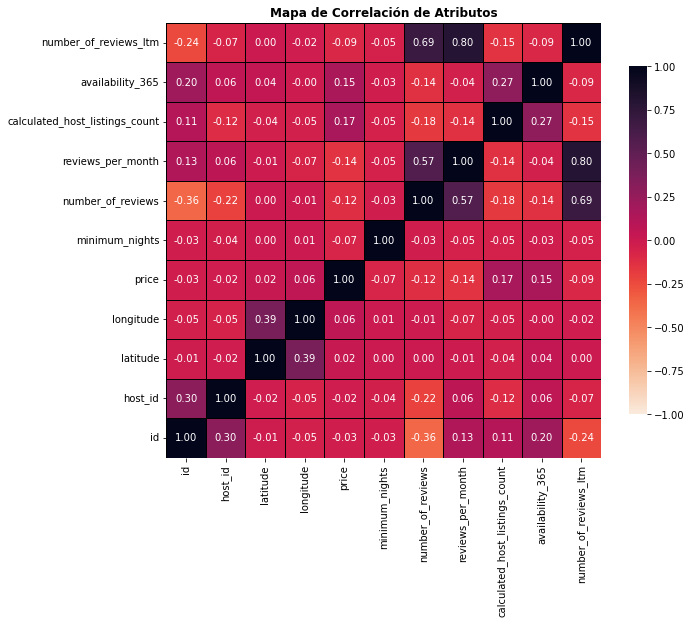
\includegraphics[width=0.9\textwidth]{capturas/25.png}
    \captionof{figure}{Mapa de correlación de atributos.}
\end{center}
Al analizar el mapa de correlación, se destacan varias conclusiones clave. La alta correlación entre el ID del alojamiento y el host\_id sugiere que ciertos anfitriones pueden tener múltiples propiedades en el mercado de alquileres. Además, la correlación entre latitud y longitud es coherente, ya que estas dos variables están intrínsecamente relacionadas con la ubicación geográfica de las propiedades.
Es interesante observar la correlación entre el número total de reseñas (number\_of\_reviews) y la tasa de reseñas mensuales (reviews\_per\_month), lo que sugiere que las propiedades que reciben más reseñas en general también tienden a recibir más reseñas por mes. 

Sin embargo, llama la atención la baja correlación entre el número total de reseñas y el ID del alojamiento, indicando que la popularidad de una propiedad medida por el número de reseñas no necesariamente está correlacionada con su posición en la secuencia de IDs.
\newpage